\Chapter{Testek optimalizálása}
\label{ch:opt}

Érdemes megnézni, hogy egyes testeknél hogyan tudunk konvergálni különböző eloszlásokhoz.
Ehhez a \ref{sect:ratiomodification} szakaszban bemutatott heurisztikát fogjuk használni.
Addig módosítjuk a testeket, amíg az oldallapokhoz tartozó relatív hiba az általunk megadott küszöbérték alá nem esik.
Ezt a küszöböt $\chi^2$-re nézve az alábbi összefüggéssel írhatjuk fel:
\[
\begin{array}{c}
\chi^2=\sum\limits_{i=1}^{n} \frac{(e_i\cdot (1+error) - e_i)^2}{e_i} = \sum\limits_{i=1}^{n} \frac{(e_i + e_i\cdot error - e_i)^2}{e_i} = \sum\limits_{i=1}^{n} \frac{(e_i\cdot error)^2}{e_i} = \\
= \sum\limits_{i=1}^{n} \frac{e_i^2\cdot error^2}{e_i} = \sum\limits_{i=1}^{n}{e_i\cdot error^2} = error^2 \sum\limits_{i=1}^{n} e_i = error^2 \cdot N,
\end{array}
\]
ahol $e_i$ az oldalakhoz tartozó elvárt gyakoriság, $N$ a dobássorozat száma és $error$ az általunk megadott hibaküszöb.
Ezt a küszöböt tudnánk igazítani ahhoz is, hogy a módosított testet milyen szignifikancia szinten szeretnénk elfogadni.
Testenként változó, hogy egy adott $\alpha$ szignifikancia szinthez tartozó  $\chi^2$ érték maximum mennyi lehet, és annak nagysága nagyban függ a dobássorozatok méretétől, ezért a fent leírt képlettel fogjuk számolni a hibaküszöböt.

A fejezet további részében az optimalizálások kerülnek bemutatásra.
Mindegyik mérésről lesz egy leírás, hogy miért azt az eloszlást választottuk, milyen eredményre számítunk.
A testek és a várt eloszlás leírása után fognak szerepelni a futásnál használt paraméterek és a konvergencia görbe.
Végül az egyéb tapasztalatok jönnek, hogy mennyire hasonlít a test az általunk elképzelt alakzatra.

\Section{Tetraéder}

Az alap tetraéder, amit módosítani fogunk 50 egység hosszú oldallapokkal rendelkezik.
Azért, hogy a módosított alakzatokat $\alpha = 0.05$ szignifikancia szinten el tudjuk fogadni a $\chi^2 < 7.815$ feltételnek teljesülnie kell.

A módosító algoritmusok leírásánál ezen a testen végeztünk teszteket, és mindig a $[0.1, 0.2, 0.3, 0.4]$ eloszlást közelítettük.
Azért ezeket az értékeket választottuk, mert itt egyértelműen látszódik az egyes oldallapok közötti különbség, valamint könnyen meg tudjuk határozni ránézésre, hogy a mért frekvenciák mennyire térnek el az elvárt értékektől.

\begin{figure}[h!]
	\centering
	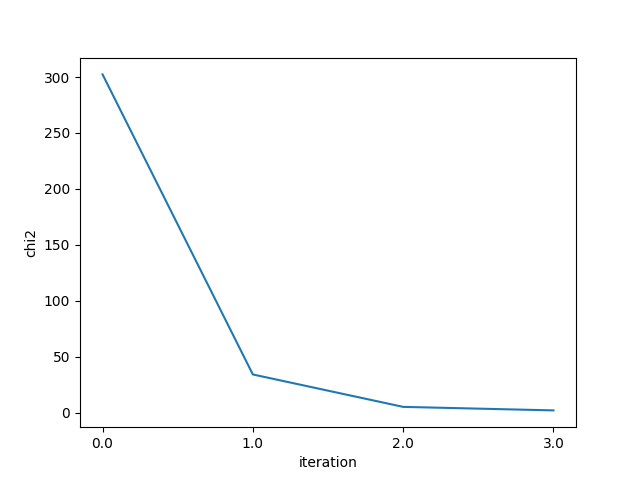
\includegraphics[scale=0.7]{images/tetrahedron_01.png}
	\caption{Az teszt eloszláshoz tartozó konvergencia görbe.}
	\label{fig:tetra01}
\end{figure}
%end chi2 = 1.9608333333333332

\begin{figure}[h!]
	\centering
	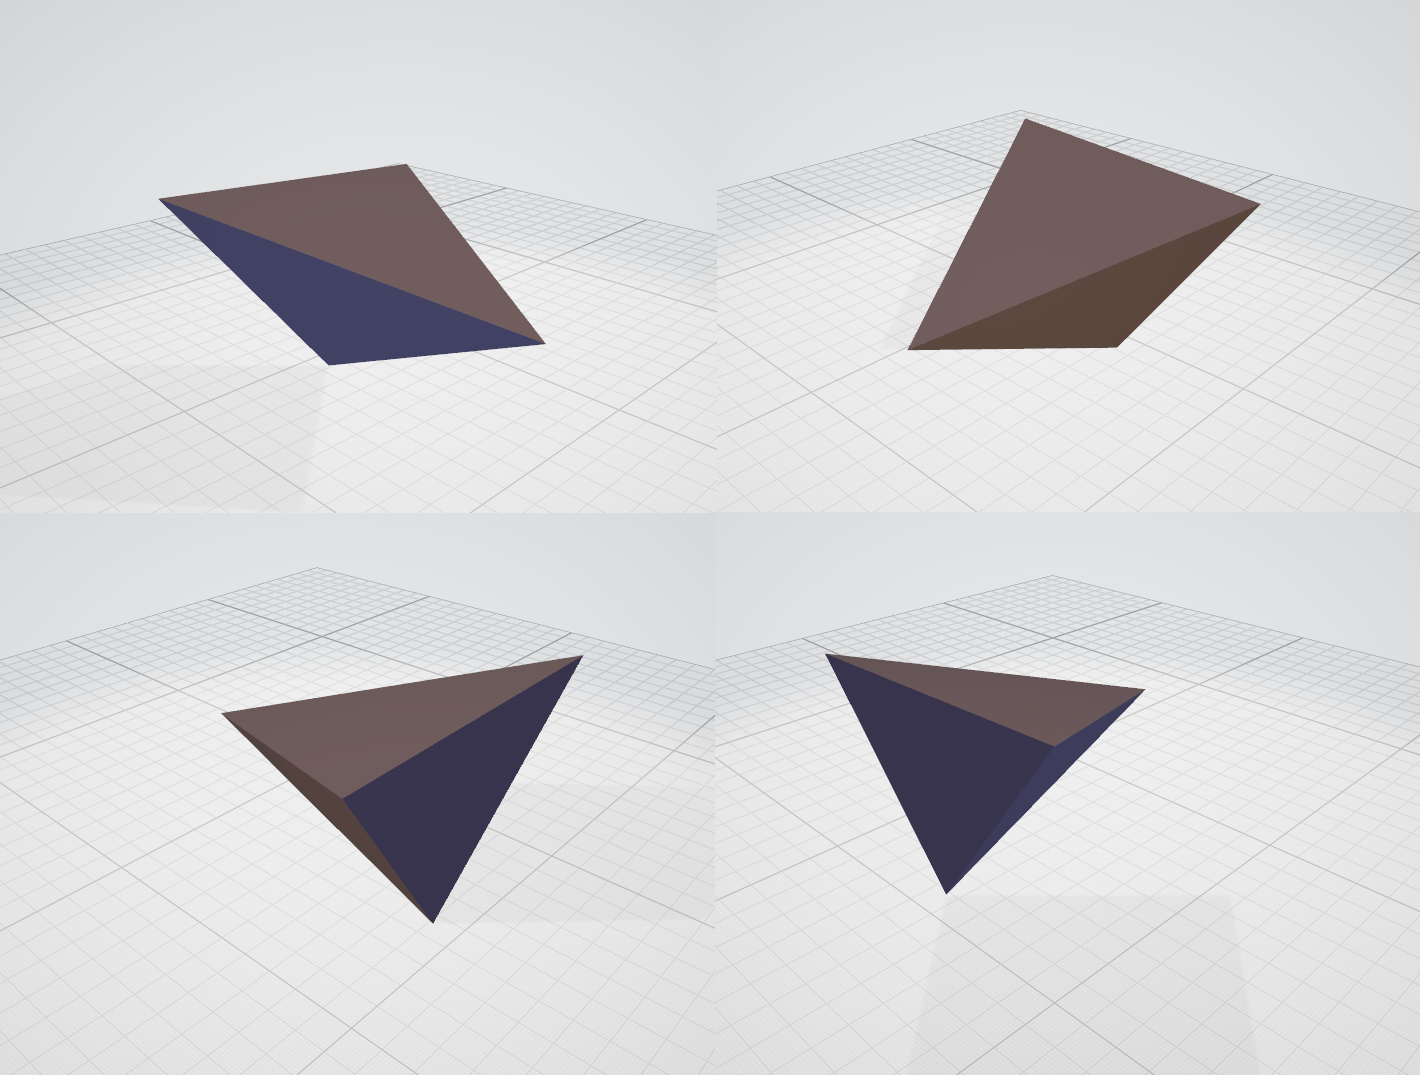
\includegraphics[width=\textwidth]{images/tetra01obj.png}
	\caption{A teszt eloszláshoz kapott alakzat.}
	\label{fig:tetra01obj}
\end{figure}

\Aref{fig:tetra01} grafikonon látható a konvergenciája a testnek az említett eloszláshoz.
Látható, hogy a választott teszt eloszlás nem csak vizsgálat szempontjából előnyös, hanem könnyen elérhető.
Az optimalizálással kapott testről láthatunk néhány képet különböző szögekből \aref{fig:tetra01obj} ábrán.

A következő test a \textit{Dark Souls: The Board Game}-ben \cite{darksouls} használt narancssárga dobókocka közelítése.
A kocka oldallapjain található értékek a következőek: 1 darab egyes, 2 darab kettes, 2 darab hármas és 1 darab négyes.
Mivel csak négy érték fordul elő, ezért lehet a testet egy tetraéderrel közelíteni, aminek várhatóan kettő oldallapja nagyobb, kettő oldallapja pedig kisebb lesz.
Így a közelítendő eloszlás: $[\frac{1}{6}, \frac{1}{3}, \frac{1}{3}, \frac{1}{6}]$.

\begin{figure}[h!]
	\centering
	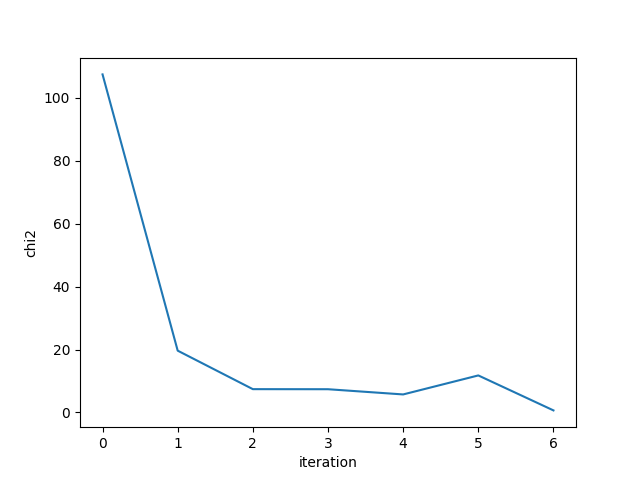
\includegraphics[scale=0.7]{images/tetrahedron_02.png}
	\caption{Az második tetraéder konvergencia görbéje.}
	\label{fig:tetra02}
\end{figure}
%end chi2 = 3.689

\begin{figure}[h!]
	\centering
	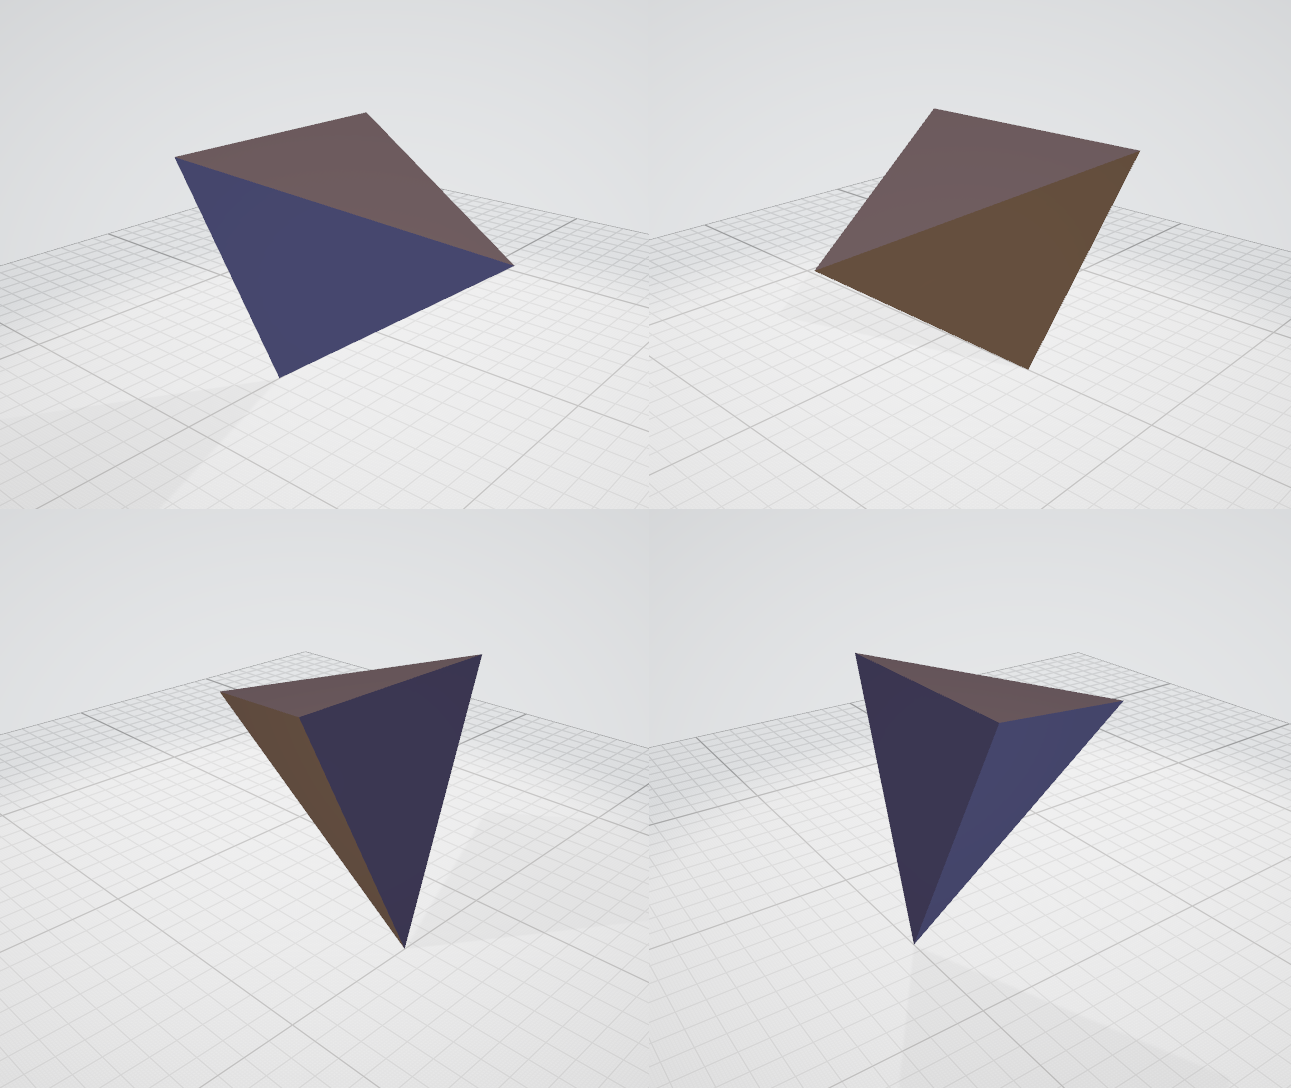
\includegraphics[width=\textwidth]{images/tetra02obj.png}
	\caption{A \textit{Dark Souls} társasjáték narancssárga dobókockájának a közelítése.}
	\label{fig:tetra02obj}
\end{figure}

\Aref{fig:tetra02} grafikonon látható, hogy a választott eloszlás elérése nem olyan triviális.
Az algoritmus követ el hibákat, amelyek a test alakja miatt nem okoznak látványos változást a görbén.

A kapott test oldallapjai egyenlő szárú háromszögekhez hasonlítanak, amelyeknek az alapjuk más hosszúságú.
Felismerhető, hogy kis hibával különböznek az egyforma lappárok, valamint az alap feltételezésünk, hogy a ritkább előfordulású oldallapok területe kisebb lesz beigazolódott.

\newpage

\Section{Dupla tetraéder}

A dupla tetraéder a sima változatához hasonlóan $50$ egység hosszú oldalélekkel fog rendelkezni.
A $\chi^2$ próbánál, hogy $\alpha = 0.05$ szignifikancia szinten el tudjuk fogadni a módosítást a $\chi^2$-nek kisebbnek kell lennie mint $11.07$.

A tetraéderhez hasonlóan egy egyszerűbbnek tűnő eloszlással fogunk kipróbálni.
Az eloszlás:
\[
\left[\frac{1}{12}, \frac{2}{12}, \frac{3}{12}, \frac{3}{12}, \frac{2}{12}, \frac{1}{12}\right].
\]

\begin{figure}[h!]
	\centering
	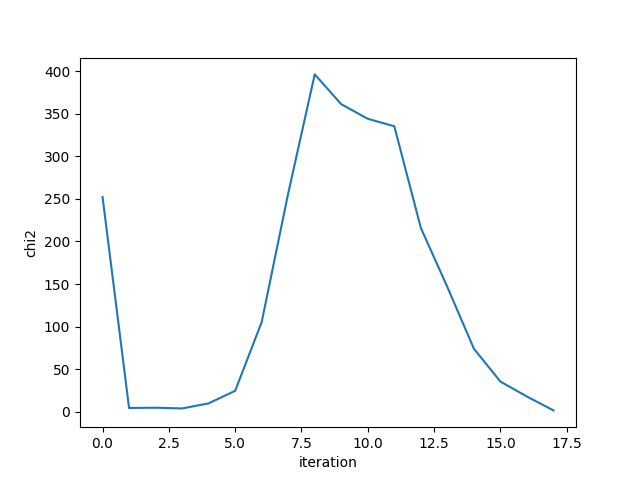
\includegraphics[scale=0.7]{images/doubletetrahedron_01.png}
	\caption{Az első dupla tetraéder konvergencia görbéje.}
	\label{fig:doubletetra01}
\end{figure}
%after test chi2 = 1.9919999999999995

\begin{figure}[h!]
	\centering
	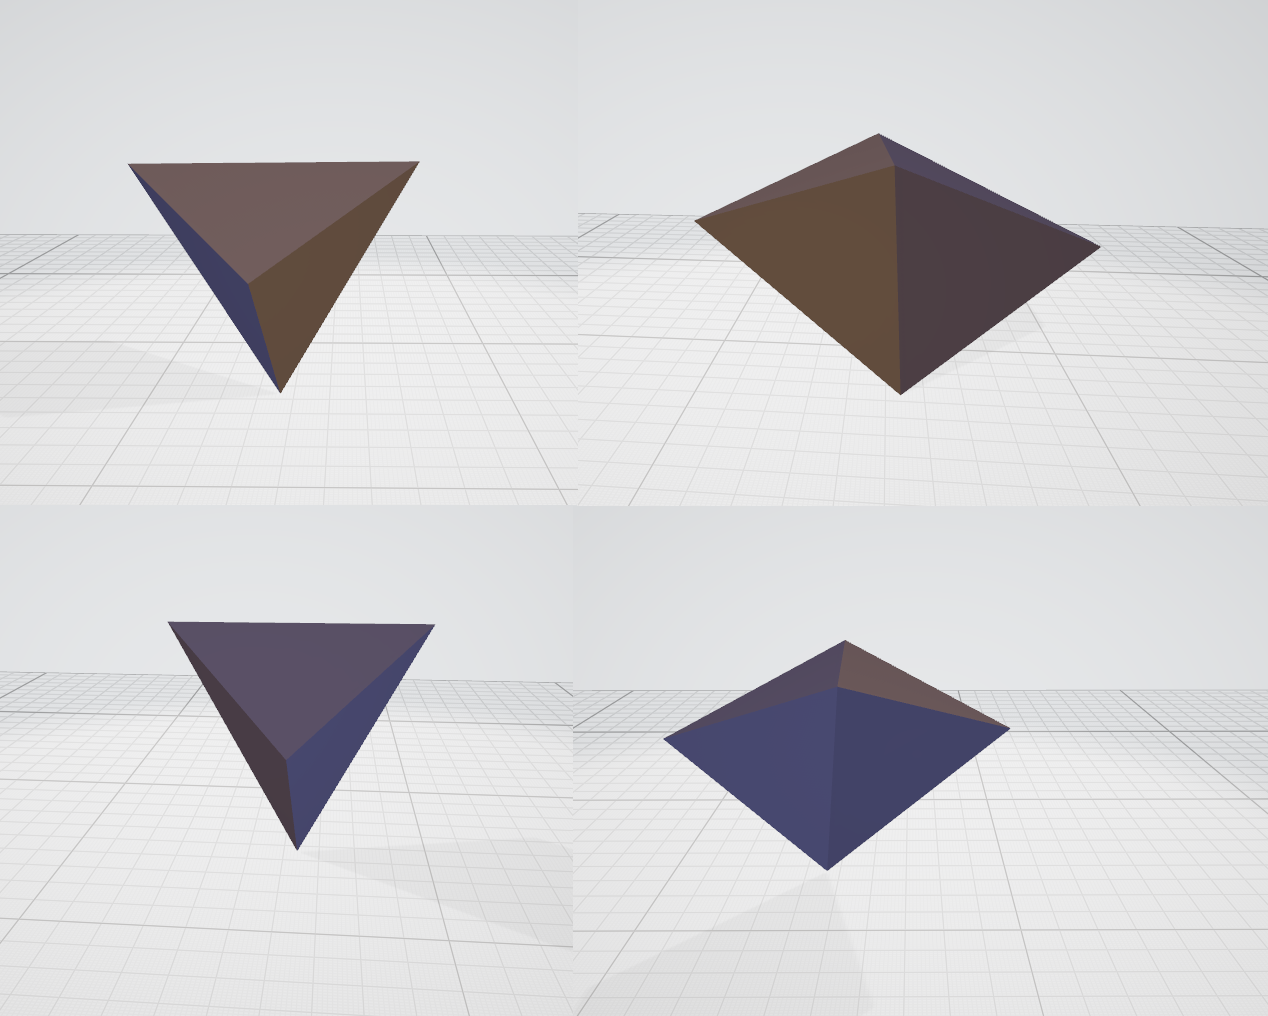
\includegraphics[width=\textwidth]{images/double01obj.png}
	\caption{Az első dupla tetraéder.}
	\label{fig:double01obj}
\end{figure}

\Aref{fig:doubletetra01} grafikonon látható, hogy az 5. iterációtól kezdve elkezdett az algoritmus egyre rosszabb értékeket kapni, és csak utána tudott a megfelelő értékhez konvergálni.
Ez amiatt történt, hogy a $\chi^2$ érték nagyon közel került a küszöbértékhez, és a következő iterációkban lévő fokozatos romlás a $\lambda$ értéknek köszönhető.
Ilyen esetekre számítottunk amikor \aref{sect:ratiomodification} szakaszban a $\lambda$ értéket akartuk meghatározni.

A következő módosításnál a
\[
\left[\frac{2}{15}, \frac{2}{15}, \frac{2}{15}, \frac{2}{15}, \frac{2}{15}, \frac{1}{3}\right]
\]
eloszlást szeretnénk elérni.
Arra számítunk, hogy egy olyan "cinkelt" testet kapunk, amelyen az egyik oldal az esetek harmadában lesz a dobások eredménye, a maradék öt oldalnak pedig az előfordulása egyenletes lesz a fennmaradó valószínűségre nézve.

\begin{figure}[h!]
	\centering
	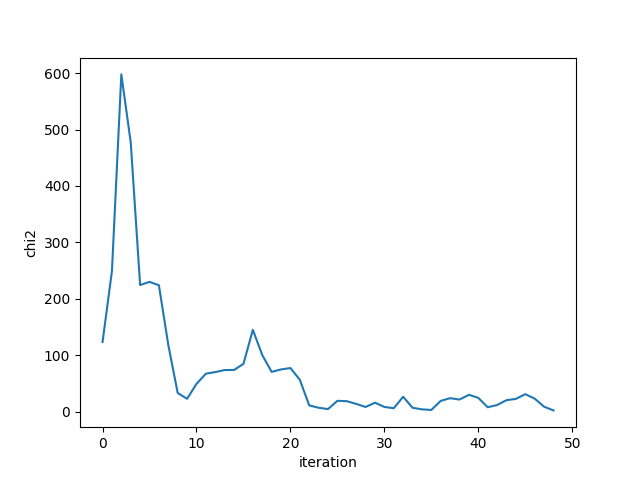
\includegraphics[scale=0.7]{images/doubletetrahedron_02.png}
	\caption{A második dupla tetraéder konvergencia görbéje.}
	\label{fig:doubletetra02}
\end{figure}
%after test chi2 = 9.489499999999996

\begin{figure}[h!]
	\centering
	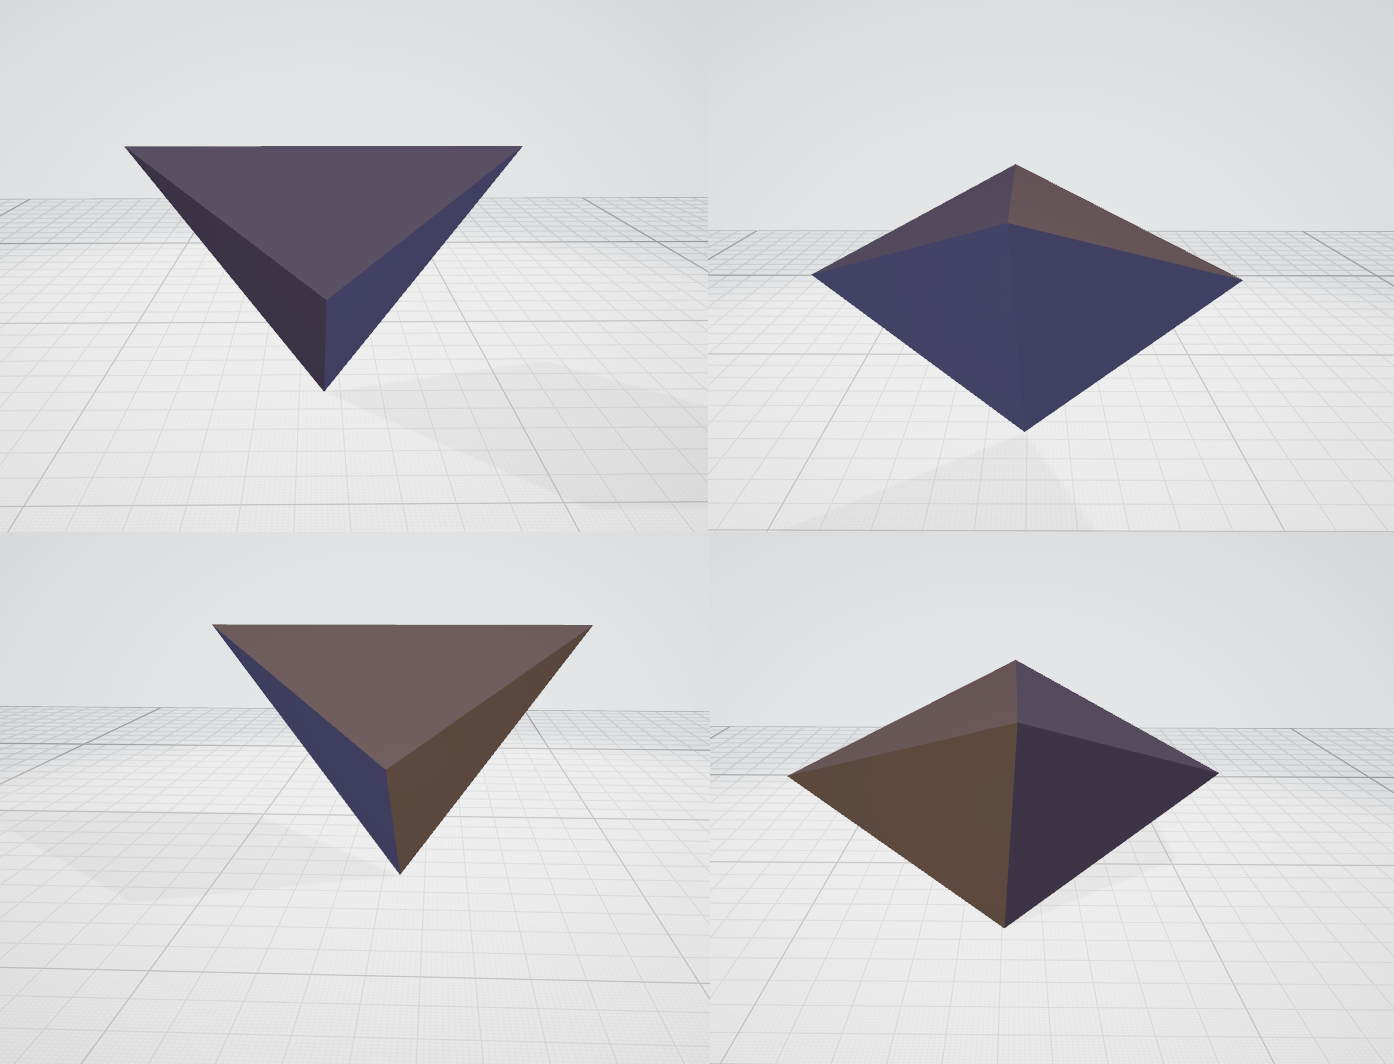
\includegraphics[width=\textwidth]{images/double02obj.png}
	\caption{A második dupla tetraéder.}
	\label{fig:double02obj}
\end{figure}

\Aref{fig:doubletetra02} grafikon az előzővel ellentétben nem mutatott extrém eltéréseket, de sokkal nehezebben tud konvergálni az elvárt értékekhez.
A kapott testen nem olyan látványos az oldallapok közötti különbség mint amire számítottunk.

\newpage

\Section{Oktaéder}

A kezdeti oktaéder csúcsai a középpontjától 50 egység távolságra helyezkednek el, így az oldalélek kicsivel nagyobbak az előzőleg tesztelt testekénél.
A könnyebb inicializálás miatt választottuk a méretének ezen meghatározását.
Az ellenőrzésnél a $\chi^2 < 14.067$ vizsgálatnak kell teljesülnie.

\begin{remark}
A szimulációkban nagyobb hibaküszöböt használunk, mert a test alakja miatt nehezebben közelíthető az eloszlás.
A mintaszámot is növelhetnénk, de akkor a futási idő exponenciálisan nőne.
\end{remark}

Az első testtel a hét érme feldobása során kapott értékek összegét szeretnénk közelíteni.
(Az érmedobás eredményét nullának vagy egynek vesszük.)
A várt binomiális eloszlás: 
\[
[\frac{1}{128}, \frac{7}{128}, \frac{21}{128}, \frac{35}{128}, \frac{35}{128}, \frac{21}{128}, \frac{7}{128}, \frac{1}{128}].
\]

\begin{figure}[h!]
	\centering
	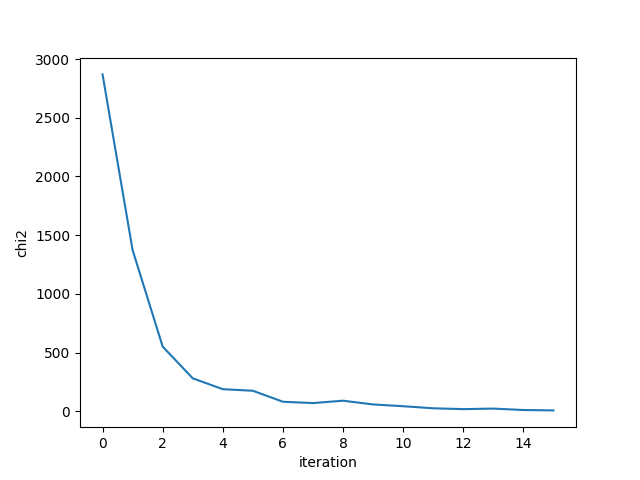
\includegraphics[scale=0.7]{images/octahedron_01.png}
	\caption{Az első oktaéder konvergencia görbéje.}
	\label{fig:octa01}
\end{figure}
%after test chi2 = 65.54
% wrong

\begin{figure}[h!]
	\centering
	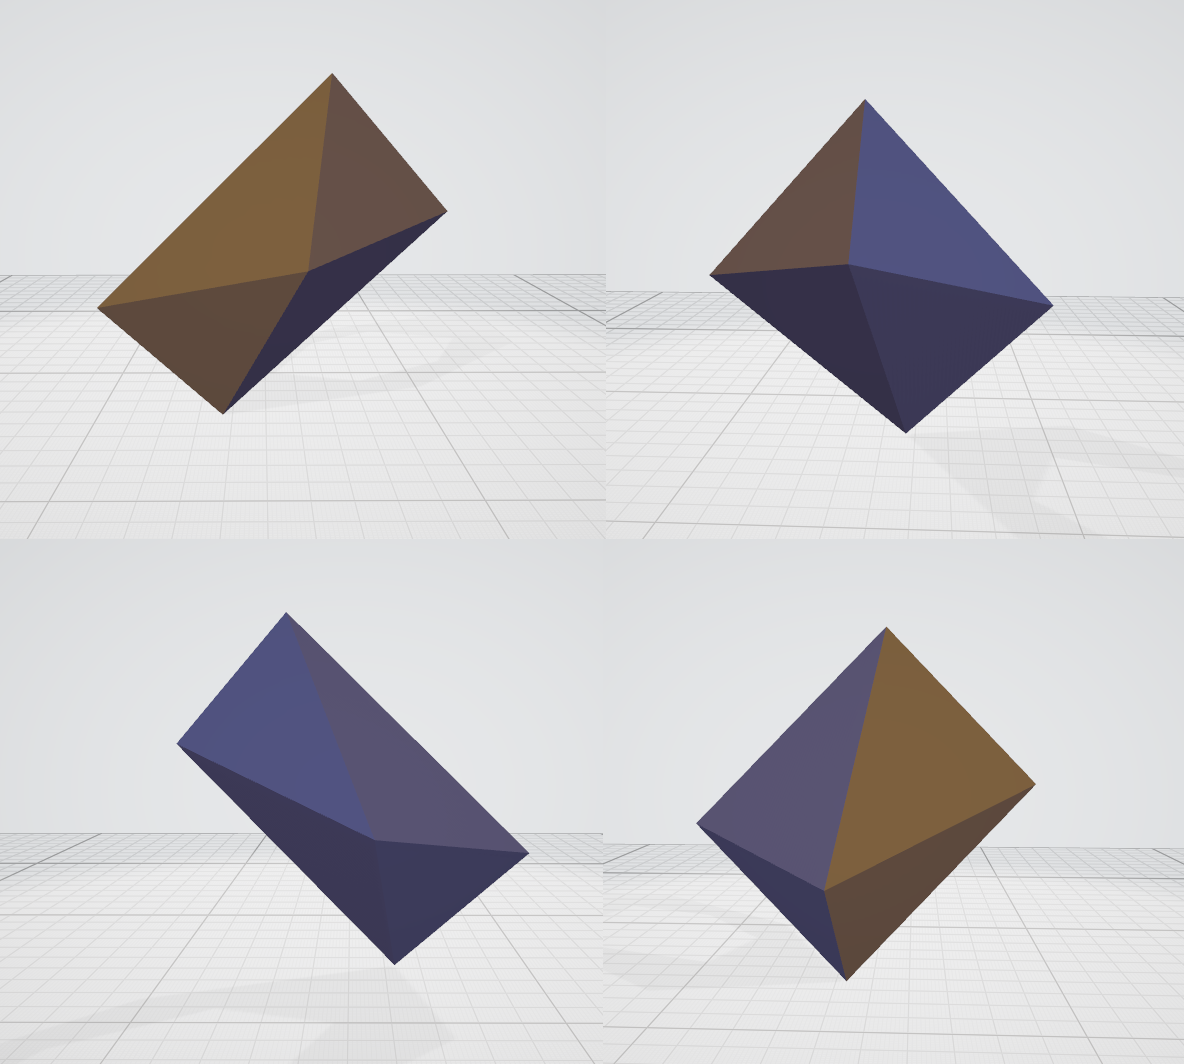
\includegraphics[width=\textwidth]{images/octa01obj.png}
	\caption{Az első oktaéder.}
	\label{fig:octa01obj}
\end{figure}

\Aref{fig:octa01} grafikonon látható konvergencia alapján ez a legjobb eredmény amit a mérések alatt kaptunk.
Ezzel ellentétben az algoritmus leállása után végzett $\chi^2$ próbán nem felelt meg nekünk a test.
Ez annak a következménye, hogy az elvárt eloszlás nehezen közelíthetősége miatt feljebb vittük a hibaküszöböt, és így pontatlanabb mérést kaptunk.
A Python kódok lassú futási ideje miatt nem a mintavételt növeltük.

Mivel az egyes valószínűségek rögzítve vannak az oldallapokhoz, így meg tudjuk adni azt, hogy két szemben lévő lapnak nagyobb legyen az előfordulása.
Arra számítunk hogy a kapott testnek az alakja kicsit hasonlítani fog egy hasábra.
A várt eloszlás:
\[
[\frac{1}{4}, \frac{1}{12}, \frac{1}{12}, \frac{1}{12}, \frac{1}{12}, \frac{1}{12}, \frac{1}{12}, \frac{1}{4}].
\]

\begin{figure}[h!]
	\centering
	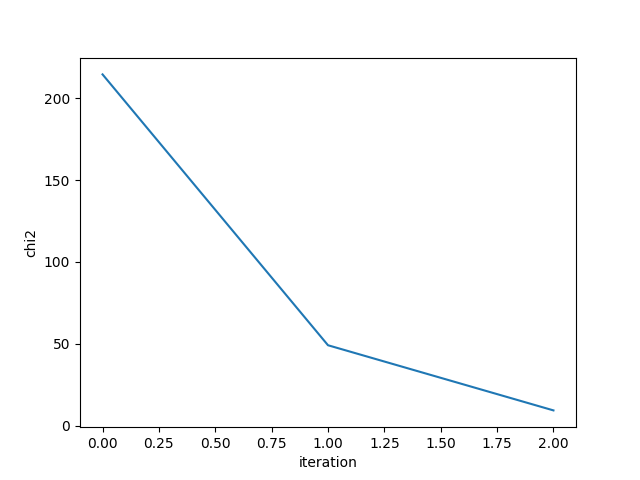
\includegraphics[scale=0.7]{images/octahedron_02.png}
	\caption{A második oktaéder konvergencia görbéje.}
	\label{fig:octa02}
\end{figure}
%after test chi2 = 7.92

\begin{figure}[h!]
	\centering
	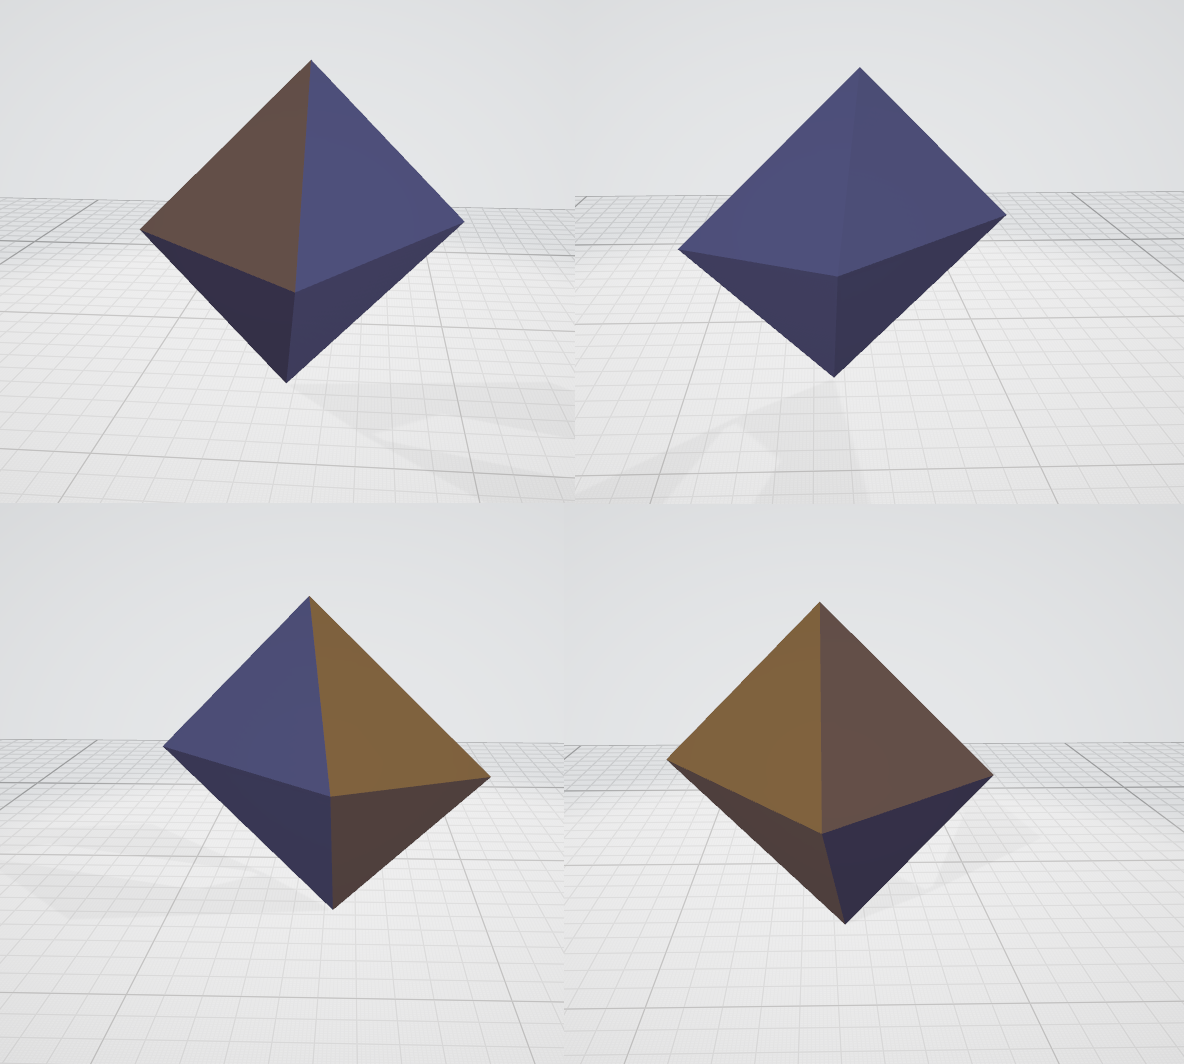
\includegraphics[width=\textwidth]{images/octa02obj.png}
	\caption{Az második oktaéder.}
	\label{fig:octa02obj}
\end{figure}

\Aref{fig:octa02} grafikonról leolvasható, hogy egyszerűbben el tudunk jutni ehhez az eloszláshoz, mint az előtte választotthoz.
Ez itt azt bizonyítja, hogy maga az eloszlás is nagy szerepet játszik a konvergencia gyorsaságában.
A kapott testen látható (\ref{fig:octa02obj} ábra), hogy nem kaptunk annyira drasztikusan eltérő testet, mint vártuk.
A későbbiekben érdemes lehet egy szélsőségesebb eloszlást kipróbálni.